\chapter{三点估算} % Introduction chapter suppressed from the table of contents

\hypertarget{ux4f30ux7b97ux662fux4e00ux4e2aux8303ux56f4ux4e0dux662fux4e00ux4e2aux6570}{%
\subsection{估算是一个范围,不是一个数}\label{ux4f30ux7b97ux662fux4e00ux4e2aux8303ux56f4ux4e0dux662fux4e00ux4e2aux6570}}

唐工:你估计完成开发用户登录模块要多少天?\\
小李:3天。\\
唐工:能在3天完成的可能性有多高?\\
小李:可能性很高。\\
唐工:可否量化一点?\\
小李:可能性为50\%~60\%。\\
唐工:所以很有可能不止3天,要4天了。\\
小李:对的,其实也有可能要5、6天,但我估计机会不大。\\
唐工:你信心有多少?\\
小李:难说,有95\%的信心可以在6天之内完成。\\
唐工:所以有可能要用上7天了?\\
小李:这样说吧,如果所有可能出问题的都出了问题,甚至会10天或11天,但这种概率很低。\\
唐工再问小李:是能否给我一个确实能完成这个模块的日期?\\
小李:正如我前面说,很可能3天可以完成,但有可能4天。\\
唐工追问:你可以说4天吗?\\
小李:也有可能5、6天。\\
唐工结束对话:OK,请你尽力6天之内完成这个模块。\\
唐工貌似请求,但实际是要求小李承诺这个模块要在六天之内开发完。假如这个模块的开发时间超过6天,唐工就有依据说小李没有尽力导致延误了。\\
所以从以上对话,可以看到作为开发专业人员,必须分清估算和承诺。作为专业人士,我们不应该给一些没有把握的承诺,误导对方。中国老话说"一诺千金"就是这个道理。

\hypertarget{ux4eceux5355ux70b9ux5230ux4e09ux70b9ux4f30ux7b97}{%
\subsection{从单点到三点估算}\label{ux4eceux5355ux70b9ux5230ux4e09ux70b9ux4f30ux7b97}}

从上面的例子可以看到,一般的单点估算是很容易被误导,以为那个天数是有把握达成的,所以我们最好从单点估算变成三点估算,除了估算最可能的天数,还有最佳和最差共三点。但项目是由一系列的任务组成(如第二任务依赖于第一个任务的完成),如何计算所有任务的总天数?
下面用例子说明如何用3种使用三点估算估计的方法(A、B、C)估算总天数:\\
A)假定都是正态分布,用模型估计:\\
先用PERT方程式计算每一步的预计值 与 标准差:\\
预计值 (Expected Value EV) = (Best + 4xMost Likely + Worst ) /6\\
标准差 (Sigma)= (Worst - Best) / 6\\

%Screenshotfrom2023-11-1221-23-06.png

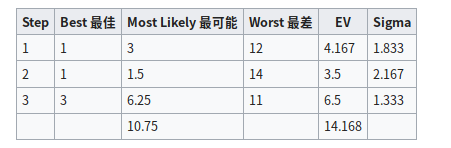
\includegraphics[width=6cm]{Screenshotfrom2023-11-1221-23-06.png}

如果假定是正态分布,按以上预计值和标准差,使用蒙特卡洛模拟,从下图可看到,95\%置信区间是
8.02 \textasciitilde{} 20.37\\
%\url{文件:pert3.1.png}

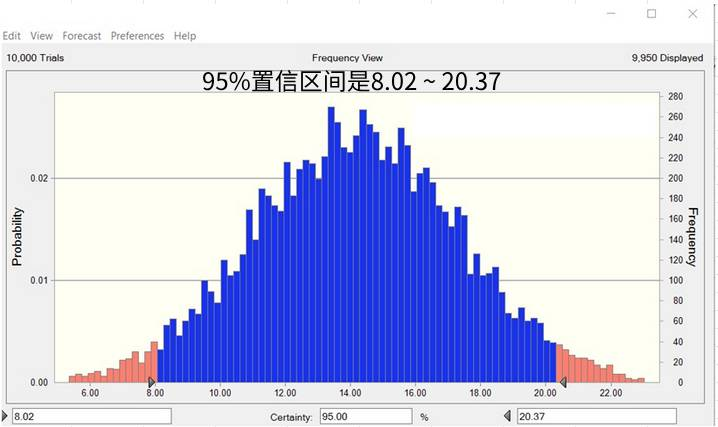
\includegraphics[width=6cm]{微信图片_20240117093405.jpg}

B) 直接用PERT方程式计算总天数的均值与标准差:\\
如不用模拟,直接把3步的均值加起来:\\
4.2 + 3.5 + 3.6 = 14\\
计算3步总方差:(方差 = \(Sigma^2\))\\
假定: 总方差 = 每步方差的总和\\
总方差 = 9.77\\
Sigma \(\sigma\)= 3.13\\
95\%置信区间计算公式为:均值的总和
\(\pm 2 \sigma = (4.2 + 3.5 + 3.6) \pm 2 x 3.13  = 14 \pm 6.26\)= 7.74
\textasciitilde{} 20.26\\
结果与蒙特卡洛模拟预测类似。\\
C) 假定都是三角形分布,用模型估计:\\
如果用三角形分布,95\%置信区间是 10.38 \textasciitilde{} 26.45\\
%\url{文件:pert32.png}

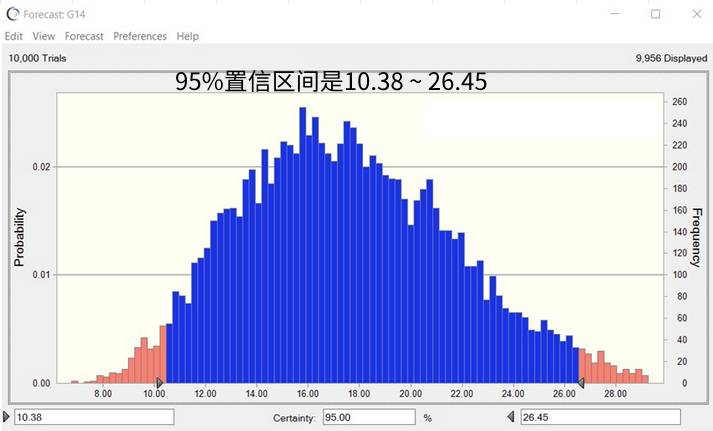
\includegraphics[width=6cm]{微信图片_20240117093446.jpg}

\hypertarget{ux603bux7ed3-ux89e3ux8bfbux5206ux6790ux7ed3ux679c}{%
\subsection{总结 +
解读分析结果}\label{ux603bux7ed3-ux89e3ux8bfbux5206ux6790ux7ed3ux679c}}

\begin{itemize}
\tightlist
\item
  如果假定每一步的分布都是一个正态分布,就可以用头两个方程式计算每一步的平均值跟标准差和方差,用方程式可计算3步的总均值大概是14。也可以用方程式计算标准差,总的标准差(sigma)是3.13左右。
  
\item
  也可用蒙特卡洛模型(假定步骤都是正态分布),得出很类似的正态分布,总的平均也接近14,95\%的置信区间是从8.02~ 20.37,
  接近上面算出的均值 \(\pm\) 两个标准差数值。
\item
  但因3个步骤都是明显往右偏,所以不能假设它们是正态分布,更合适的是使用三角形分布,然后用蒙特卡洛估算``加''起来的分布,看见最后的图明显是类似往右有个尾巴,能更正确反应3个步骤加起来的天数的估计分布。
\item
  跟假定正态分布的结果比较,很明显看到用三角形分布结果往右偏,上限是
  26.45(比正态分布的20.37
  高)。不是正态分布的话,左面就没有长尾巴,所以就会比本来正态分布的下限高,下限是
  10.38 (比正态分布的 8 高)。
\item
  从这简单例子看到,如果我们要把三点估算加起来,尤其是非正态分布的话,就不能用简单的方程式,或者假定它是正态分布来计算,需要用蒙特卡洛模型假设三角形分布才能真正反应总体的分布。\\
\end{itemize}

从这3个偏左分布步骤例子看起来好像有些偏差,但不是很严重。如果我们看见用十个步骤都是偏一边分布,总分布会如何?是否相差会更远?

\hypertarget{ux5229ux7528ux8499ux7279ux5361ux6d1bux6a21ux62df10ux4e2aux6b65ux9aa4ux4e09ux89d2ux5f62ux5206ux5e03ux7684ux603bux5206ux5e03}{%
\subsection{利用蒙特卡洛模拟10个步骤(三角形分布)的总分布}\label{ux5229ux7528ux8499ux7279ux5361ux6d1bux6a21ux62df10ux4e2aux6b65ux9aa4ux4e09ux89d2ux5f62ux5206ux5e03ux7684ux603bux5206ux5e03}}

如果每步都估算天数,10个步骤的 总天数就是500天 (把10个估算值加起来)。

但如果每个步骤都是三点估算:

%Screenshotfrom2023-11-1221-25-44.png

%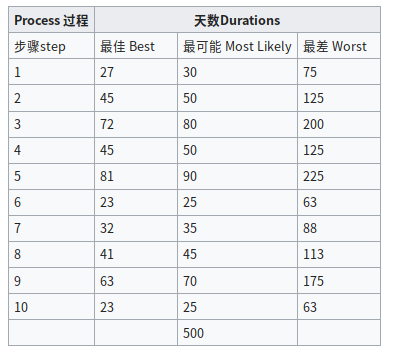
\includegraphics[width=6cm]{Screenshotfrom2024-01-1621-07-15.png}

\begin{tabular}{|c|c|c|c|}
\hline
Process 过程&\multicolumn{3}{c|}{天数Durations}\\
\hline
1&27&30&75\\
\hline
2&45&50&125\\
\hline
3&72&80&200\\
\hline
4&45&50&125\\
\hline
5&81&90&225\\
\hline
\end{tabular}

很明显看到每一步都是偏左的分布,所以可预计总天数应不止500天,
但估多少才合适?

假定每步骤是三角形分布,用模型估计重复5000次,得出下面分布:

%\href{文件:HMTT_v1.3_s77.png}{400px}

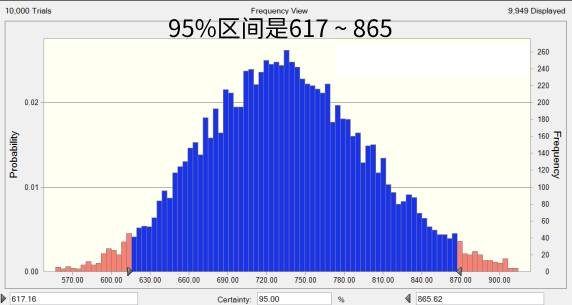
\includegraphics[width=6cm]{微信图片_20240117093538.jpg}

%Screenshotfrom2023-11-1221-27-17.png

%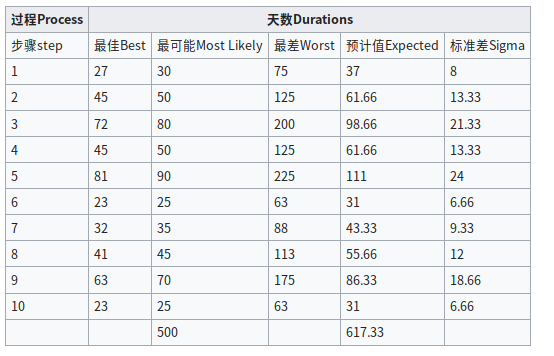
\includegraphics[width=6cm]{Screenshotfrom2023-11-1403-10-57.png}

%try CSDN LaTeX (table) code
\begin{tabular}{|c|c|c|c|c|c|}
\hline
Process 过程&\multicolumn{4}{c|}{天数Durations}\\
\hline
1&27&30&75&37&80\\
\hline
2&45&50&125&61.66&13.33\\
\hline
3&72&80&200&98.66&21.33\\
\hline
4&45&50&125&61.66&13.33\\
\hline
5&81&90&225&111&24\\
\hline
6&23&25&63&31&6.66\\
\hline
7&32&35&88&43.33&9.33\\
\hline
8&41&45&113&55.66&12\\
\hline
9&63&70&175&86.33&18.66\\
\hline
10&23&25&63&31&6.66\\
\hline
\:&\:&500&\:&617.33&\: \\
\hline
\end{tabular}

A) 用PERT方程式计算每一步的预计值 与 标准差:

%\href{文件:10stepsPertScreenshot_2022-10-24_205007.jpg}{500px}

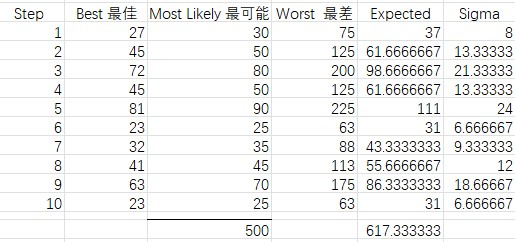
\includegraphics[width=6cm]{10stepsPertScreenshot_2022-10-24_205007.jpg}

得出95% 区间是 525.3 ~ 709.3 (= 617.3  ±  92 )

B) 假定是正态分布,按以上预计值和标准差,使用蒙特卡洛模拟,得出的总分布的结果几乎一致,都是左右平均分布的正态形。

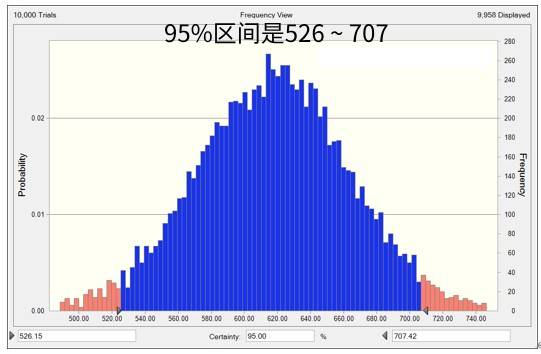
\includegraphics[width=6cm]{微信图片_20240117093606.jpg}

\hypertarget{ux5206ux679010ux6b65ux9aa4ux6a21ux62dfux7ed3ux679c}{%
\subsection{分析10个步骤模拟结果}\label{ux5206ux679010ux6b65ux9aa4ux6a21ux62dfux7ed3ux679c}}

\begin{itemize}
\tightlist
\item
  为什么用三角形分布模拟出来不是偏左的分布(类似前面3步结果),而是一个正态分布。
\end{itemize}

\begin{description}
\tightlist
\item[]
以上实验验证了“中心极限定理”,无论本来是什么形状的分布,如果随机抽样够多,样本的平均值分布接近正态分布。所以如果本来只是3个步骤的时候还是可以看出是三角形偏左,但到了用10个步骤相加时,得出的分布便非常接近正态分布。

(中心极限定理会在后面数据分析里用上,例如通过画控制图判断过程是否稳定)。\\
\end{description}

\begin{itemize}
\tightlist
\item
  实验结果也验证了当每一步都类似正态分布可以用PERT公式计算每一步的预计值和标准差,然后计算总结果的分布(不需要蒙特卡洛模拟),但如果非正态分布(如偏左的三角形分布)便需要使用蒙特卡洛模拟,不然预估会有偏差(类似上面3步模拟的结果)。
\end{itemize}

\hypertarget{ux4eceux5355ux70b9ux5230ux4e09ux70b9ux4f30ux7b97}{%
\subsection{问答 Q\&A}\label{ux4eceux5355ux70b9ux5230ux4e09ux70b9ux4f30ux7b97}}

问:为什么要花这么多精力去研究分布,我们日常不都是单点估算吗?

答:例如你觉得把整个公司的人均生产率从1.14一年后提升到1.21算不错吗?(注)
问:不是非常好,还算可以。\\
答:如果本来的分布和提升后的目标是如下图,你觉得怎么样?\\

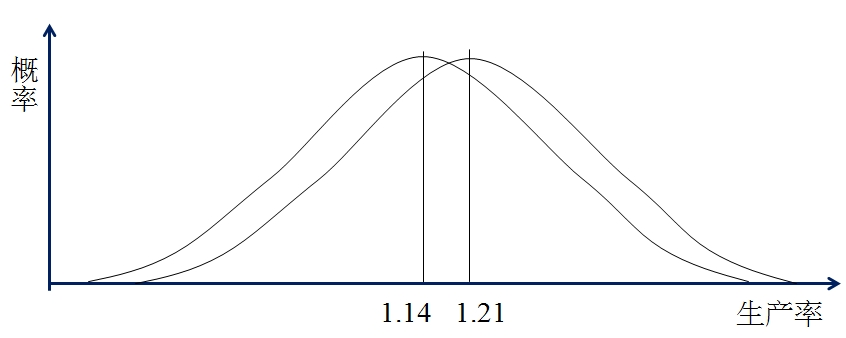
\includegraphics[width=6cm]{4_三点估算问与答1.jpg}

问:提升就太微小了。\\
答:从这简单例子看到所有估算都应包含两部分:分布和中间趋势(例如平均值)。\\
另一例子:假如我们预估生产率的分布是如下图,达到或超越1.14这目标的概率是65%:\\

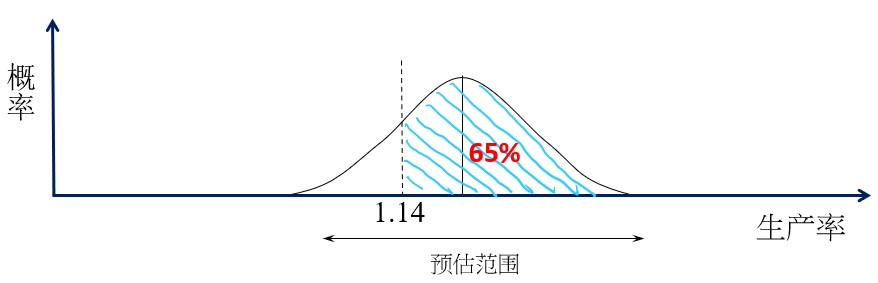
\includegraphics[width=6cm]{4_fig2a_2024-01-15_211344.jpg}

但如果告诉你目标是1.14只是目标平均值,分布是如下图:\\

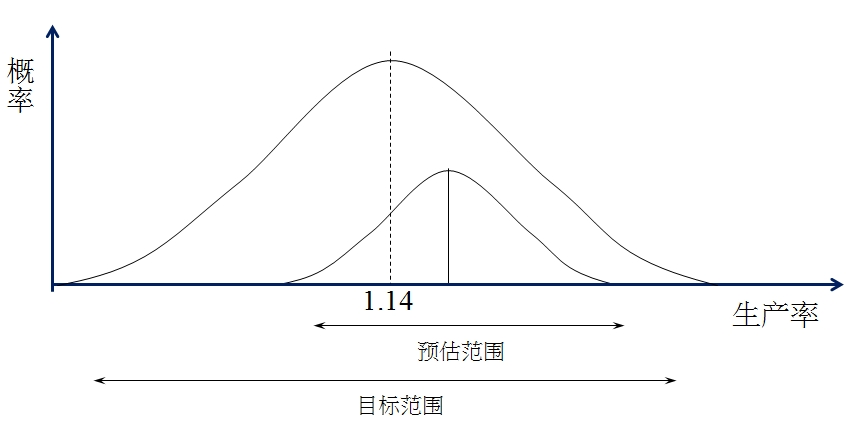
\includegraphics[width=6cm]{4_三点估算问与答2.jpg}

预测的生产率分布完全在目标范围之内。\\
(注:生产率单位 每人天产出代码的功能点数,类似有效代码行数都是衡量软件规模的单位。)\\
在下一部分,我们会看到如何使用PERT三点估算的实例。

\hypertarget{ux9644ux4ef6}{%
\section{附件}\label{ux9644ux4ef6}}

\hypertarget{ux8499ux7279ux5361ux6d1bmonte-carlo-ux6a21ux62df}{%
\subsection{蒙特卡洛(Monte Carlo)
模拟}\label{ux8499ux7279ux5361ux6d1bmonte-carlo-ux6a21ux62df}}

当结果不能用数学公式计算的时候(例如是三角形分布),可以用电脑随机模拟结果。例如:

\begin{itemize}
\tightlist
\item
  计算3个步骤的总共人天,每个步骤都是三角形分布,我们就用电脑的随机功能模拟,让随机功能的结果按三角形分布。
\item
  第一次模拟:步骤1得出1.3,步骤2得出1.2,步骤3得出2.0,得出3个步骤的总工期是4.5人天。
\item
  第二次模拟:步骤1得出1.5,步骤2得出1.15 ......。
\item
  如果我们模拟1000次、10000次,便能模拟出总分布。
\item
  因为是电脑随机模拟,出来的结果会有些偏差,但差异不会太大。(例如上面10步三角形分布的模拟结果偏差都没有低于0.3%)
\end{itemize}


